\documentclass{beamer}

\usepackage[utf8]{inputenc}
\usecolortheme{beaver}
\usepackage{caption}
\usepackage{subcaption}
\usepackage{mathtools}
\usepackage{todonotes}
\usepackage{amsmath}
\usepackage{bm}
\usepackage{listings}
\usepackage{ragged2e}
\usepackage{titlecaps}
\usepackage{fancyvrb}

\def\ci{\perp\!\!\!\!\!\perp}

\newtheorem{proposition}{Proposition}
\Addlcwords{for a is but and with of in as the etc on to if}

\setbeamertemplate{section in toc}{\inserttocsectionnumber.~\inserttocsection}
\usetheme{Boadilla}
\makeatletter
\setbeamertemplate{footline}{%
    \leavevmode%
    \hbox{%
        \begin{beamercolorbox}[wd=.3\paperwidth,ht=2.25ex,dp=1ex,center]{author in head/foot}%
            \usebeamerfont{author in head/foot}\insertshortauthor\expandafter\beamer@ifempty\expandafter{\beamer@shortinstitute}{}{~~(\insertshortinstitute)}
        \end{beamercolorbox}%
        \begin{beamercolorbox}[wd=.55\paperwidth,ht=2.25ex,dp=1ex,center]{title in head/foot}%
            \usebeamerfont{title in head/foot}\insertshorttitle
        \end{beamercolorbox}%
        \begin{beamercolorbox}[wd=.15\paperwidth,ht=2.25ex,dp=1ex,right]{date in head/foot}%
            \usebeamerfont{date in head/foot}\insertshortdate{}\hspace*{2em}
            \insertframenumber{} / \inserttotalframenumber\hspace*{2ex} 
        \end{beamercolorbox}}%
        \vskip0pt%
    }
\makeatother


\title[]{Enhancing and Promoting Data Simulation Capabilities of pgmpy}
\author{Ankur Ankan, Radboud University}
\date{May 8, 2024}
\begin{document}

\maketitle

\begin{frame}
	\centerline{pgmpy is a Python package for Bayesian Networks(BNs)}
\end{frame}

\begin{frame}{Applications of Bayesian Networks}
\begin{columns}
	\begin{column}{0.55\textwidth}
		\begin{itemize}
			\item \textbf{Predictive Modelling:}
				\begin{itemize}
					\item A generative model to efficiently represent joint distributions.
					\item Graphical structure adds interpretability.
				\end{itemize}
			\item \textbf{Causal Inference:}
				\begin{itemize}
					\item Edges are interpreted as causal direction.
					\item Used for causal effect estimation, application of interventions.
				\end{itemize}
		\end{itemize}
	\end{column}		
	\begin{column}{0.45 \textwidth}
		\begin{figure}
			\centering
			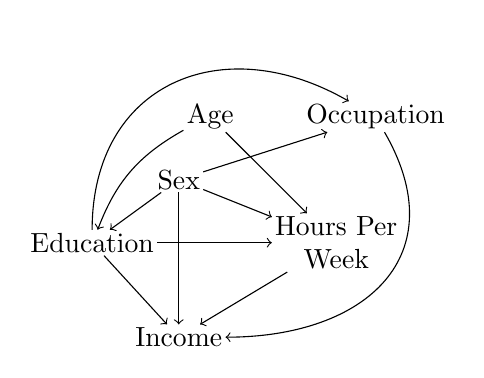
\begin{tikzpicture}[scale=1]
			\tikzstyle{every node}=[align=center, inner sep=1pt]
				\node (sex) at (-0.7, -0.8) {Sex};
				\node (age) at (-0.3, 0) {Age};
				\node (ed) at (-1.8, -1.6) {Education};
				\node (occ) at (1.8, 0) {Occupation};
				\node (hrpw) at (1.3, -1.6) {Hours Per \\ Week};
				\node (income) at (-0.7, -2.8) {Income};
			
				\draw[->]  (age) to[bend right=20] (ed);
				\draw[->]  (sex) to (ed);
				\draw[->]  (age) to (hrpw);
				\draw[->]  (ed) to (hrpw);
				\draw[->]  (sex) to (hrpw);
				\draw[->]  (ed) to (income);
				\draw[->]  (hrpw) to (income);
				\draw[->]  (occ) to[out=300, in=0, looseness=1.4] (income.east);
				\draw[->]  (sex) to (income);
				\draw[->]  (ed) to[out=90, in=150, looseness=1.3] (occ);
				\draw[->]  (sex) to (occ);	
			\end{tikzpicture}
			\caption*{\footnotesize {Example of a DAG}}
		\end{figure}
	\end{column}
\end{columns}
\end{frame}

\begin{frame}{Simulations in Bayesian Networks}
	\todo[inline]{Look into more examples how people are using simulations}
	\begin{itemize}
		\item \textbf{Predictive Modelling:}
			\begin{itemize}
				\item Approximate Inference.
				\item Validating methods such as Structure Learning.
				\item Teaching
			\end{itemize}
		\item \textbf{Causal Inference:}
			\begin{itemize}
				\item Validating methods such as causal discovery, causal estimation.
				\item Teaching.
			\end{itemize}
	\end{itemize}
\end{frame}

\begin{frame}{State of Simulation Features in pgmpy}
	Already has extensive features for simulation under various condition:
	\begin{itemize}
		\item Certain/Uncertain evidence
		\item Certain/Uncertain Intervention.
		\item Time-Series data.
		\item Partial simulations.
	\end{itemize}

	\vspace{1em}
	\begin{itemize}
		\item No other python package has such extensive simulation features.
	\end{itemize}
	\todo[inline]{List some other packages here}

	\vspace{3em}
	\centerline{\textcolor{red}{Limited to discrete variables only}}
	\centerline{Many requests to extend pgmpy to continuous variables.}

	% Allows simulation from these BNs under various conditions such as
	% (uncertain) evidence, (uncertain) intervention, time-series data,
	% partial simulations for incorporating other simulations.

	% Wide range of features but is limited to discrete variable.

	% Extending this to continuous variables would have a huge impact as it
	% would allow for  a lot of different simulations. No other Python
	% package that offers so much functionality.
\end{frame}

\begin{frame}{Emails}
\end{frame}

\begin{frame}{Fellowship Plan: Phase 1}
	Extend the simulation capabilities to continuous variables.

	%TODO: Show a figure to show the following message:

	The parameterization is represented in tabular CPDs which is essentially a function of the variable given it's parents. => Extend pgmpy such that it can accept arbitrary functions.
\end{frame}

\begin{frame}{Fellowship Plan: Phase 2}
	Promote these data simulation capabilities.

	\begin{itemize}
		\item Tutorial for the predictive modelling user. They don't need intervention, typically don't include latent variables.
		\item Tutorial for the causal inference user. Intervention, latent variables.
	\end{itemize}
\end{frame}

\begin{frame}{Why am I suitable to perform this}
	\begin{itemize}
		\item Started and maintained the package, very familiar with the ins/outs.
		\item I use simulations in my research, have an understanding of how it is used.
		\item Have an understanding of the userbase of how they use these methods.
	\end{itemize}
\end{frame}

\end{document}
